\documentclass[border=10pt]{standalone}
\usepackage{tikz}\usepackage{amsmath}\usetikzlibrary{arrows.meta,patterns}
\begin{document}
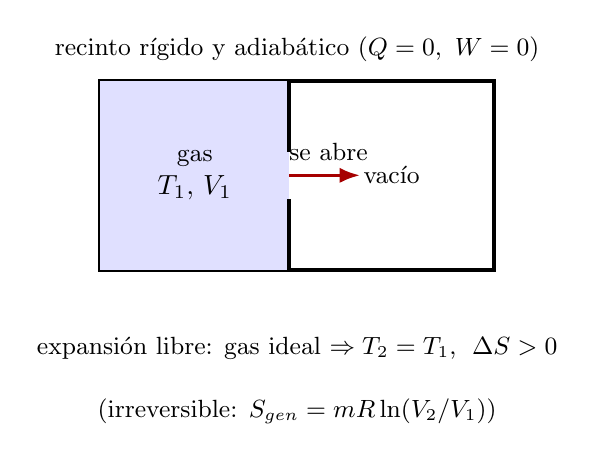
\begin{tikzpicture}[line width=1pt,>={Latex[length=2.6mm]}]
  % recinto aislado (pared gruesa)
  \draw[line width=1.6pt] (0,0) rectangle (5,2.4);
  \node at (2.5,2.8){\small recinto rígido y adiabático ($Q=0,\ W=0$)};
  % camara izquierda: gas
  \fill[blue!12] (0,0) rectangle (2.4,2.4);
  \node[align=center] at (1.2,1.2){\small gas\\$T_1,\,V_1$};
  % camara derecha: vacio
  \node[align=center] at (3.7,1.2){\small vacío};
  % valvula central
  \draw[line width=1.3pt] (2.4,0)--(2.4,0.9) (2.4,1.5)--(2.4,2.4);
  \draw[->,red!65!black,line width=1.2pt] (2.4,1.2)--(3.3,1.2);
  \node[above] at (2.9,1.25){\small se abre};
  \node[align=center] at (2.5,-1.0){\small expansión libre: gas ideal $\Rightarrow T_2=T_1$, \;$\Delta S>0$};
  \node[align=center] at (2.5,-1.8){\small (irreversible: $S_{gen}=mR\ln(V_2/V_1)$)};
\end{tikzpicture}
\end{document}
